\documentclass[10pt]{article}
\usepackage[portuguese]{babel}
\usepackage[utf8]{inputenc}
\usepackage{color}
\usepackage{enumitem}
\usepackage{float}
\usepackage{graphics}
\usepackage{minted}
\usepackage{geometry}
\geometry{
    a4paper,
    total={150mm,257mm},
}

\setlength{\arrayrulewidth}{0.3mm}
\setlength{\tabcolsep}{10pt}
% \setlength{\parindent}{0em}
\renewcommand{\arraystretch}{1.5}
\renewcommand{\thesection}{}

\begin{document}
\begin{center}
    {\scshape Instituto Superior Técnico\par}
    \vspace{1cm}
    {\scshape\Large Applications and Computation for the Internet of Things\par}
    \vspace{1.5cm}
\end{center}
{\scshape\LARGE 1\textsuperscript{st} Lab Work: Building an embedded system}
\\
\begin{table}[h!]
    \centering
    \begin{tabular}{|l|l|p{10cm}|}
        \hline
        \multicolumn{3}{|l|}{Group: XX} \\[1.5ex] \hline
        Student 1 & XXXXX & Dominika Florczykowska \\ [1.5ex]\hline
        Student 2 & 97144 & Pedro Mendes \\ [1.5ex]\hline
    \end{tabular}
\end{table}

\section{Goal:}
The goal of this work is to put students for the first time in touch with the
Arduino environment to drive simple actuators (in the case LEDs).
\section{Description:}
Build an embedded system using the Arduino UNO board to control 4 LEDs with
different colors. In normal operation, in each 5 seconds period the system will
have the the following

\begin{enumerate}
    \item Red LED ON
    \item Green LED ON
    \item Blue LED ON
    \item Yellow LED ON
    \item All LEDs OFF
\end{enumerate}

This behavior is then repeated.

The figure represents the circuit to drive the LEDs to be assembled.

\begin{figure}[H]
    \centering
    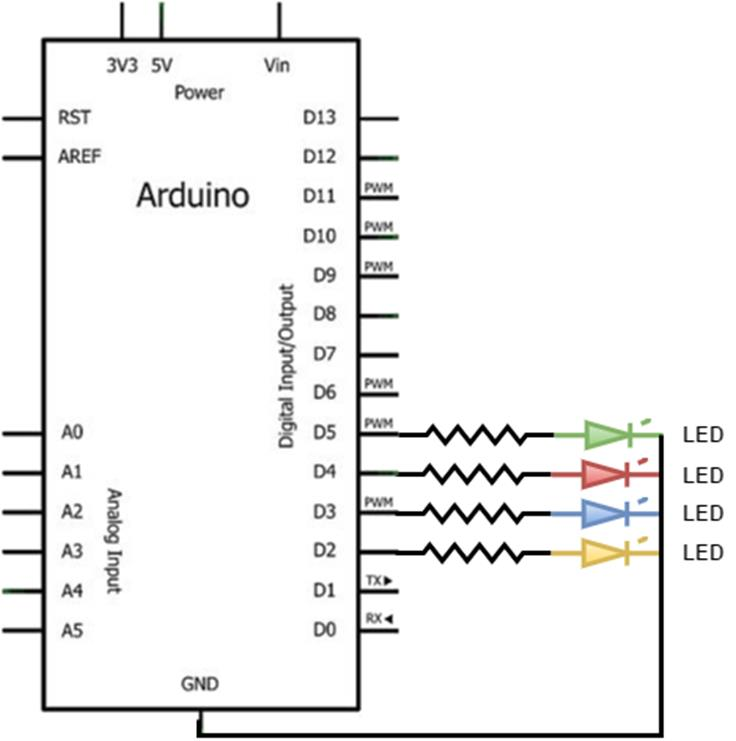
\includegraphics{arduino.jpg}
\end{figure}

\section{Design the interface}

Calculate the values of the resistors associated with the LEDs.

\begin{itemize}[label={}]
    \item R\_red
    \item R\_green
    \item R\_blue
    \item R\_yellow
\end{itemize}

Interface the circuit to a press button.

Whenever the button is pressed (OFF → ON → OFF) the LED activated at the moment must
remain ON. (In stage 5 the system stops with all LEDs OFF.) With the system stopped it is
easier to read the voltage drop on each LED. When the button is pressed again the system
will continue its normal operation sequence.

Draw and design the press button interface to the controller.

\begin{figure}[H]
    \centering
    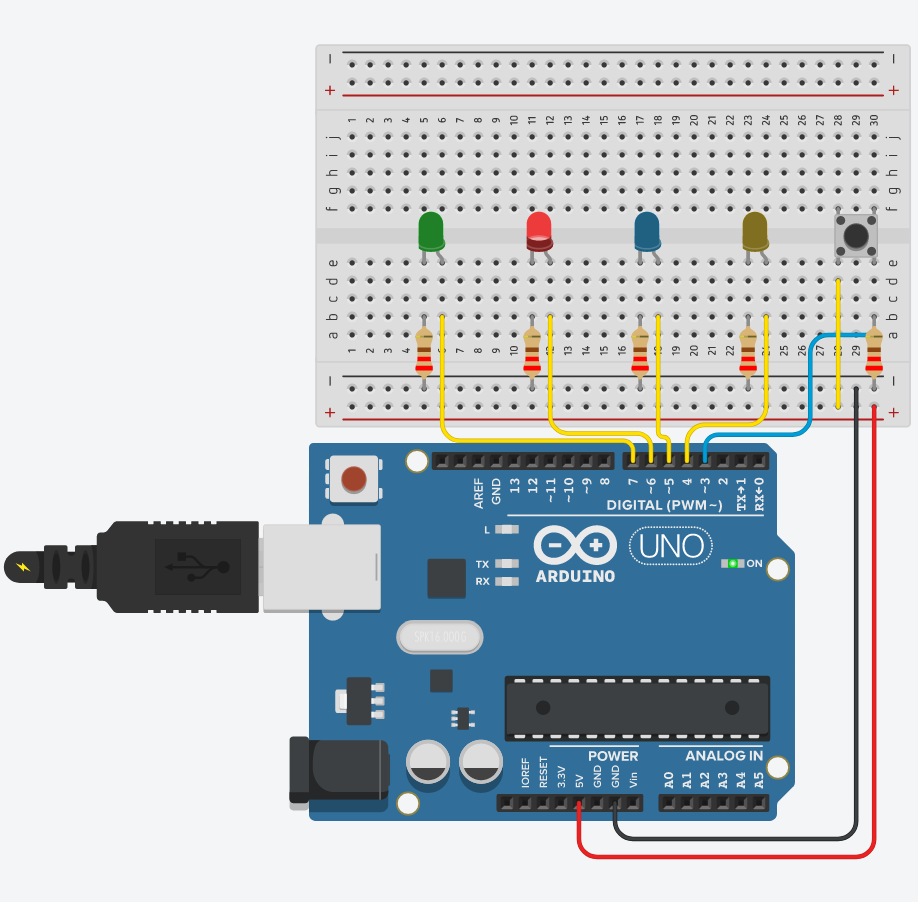
\includegraphics{button_circuit.png}
\end{figure}

Measure the voltage drops on the LEDs:

\begin{itemize}[label={}]
    \item V\_red
    \item V\_green
    \item V\_blue
    \item V\_yellow
\end{itemize}


Estimate the power consumption of the interface (the circuit with resistors and
LEDs in the figure) in normal operation.


\newpage

\section{Program de application}

\inputminted{arduino}{../lab1.ino}

\end{document}
